% !TEX root =  main.tex

\section{Introduction}

%! TEX root = ../../main.tex

\subsection{Problem Statement \& Research Goals}%
\label{sub:Problem_Statement}

Kane and Matthias suggest that \enquote{shipping software at the speed expected
in today's world is hard to do well} \autocite[p.
2]{SeanPKaneDocker&Running2018}. When implemented well, microservices can
contribute towards faster shipping software. However not only the speed at
which software is shipped these days is difficult. With the introduction of
microservices multiple new challenges arise such as how these microservices can
be monitored, scaled, optimized and orchestrated \autocite[p.
67]{TrihinasDevOpsasService2018}. Besides that, a number of security challenges
emerge when using the microservices paradigm
\autocite{YaryginaOvercomingSecurityChallenges2018}.

This thesis will mainly focus on the orchestration challenge with only one
exception. It will try to answer the question \textit{how can microservices be
continuously developed and deployed}. This question however is far too
extensive to be discussed and answered as a whole. Thus, this thesis
will focus on two \textit{problem domains} each with their own encapsulated
research question.

\label{link:problem_domains}
\begin{itemize}
  \item How should a continuously deployed microservice be versioned?
  \item How should microservice manifests be managed and continuously deployed?
\end{itemize}

The answers to these questions combined with the underlying background
information will give an overview on the landscape of microservices and how
they can be continuously developed and deployed. The goal is to help developers
and software operators to tackle the problems outlined in the research
questions above. The gained knowledge can help those who face these problems to
ship their microservice software faster and with more control.

In order to answer the question of each problem domain, the \ac{DSR} framework
will be used. Chapter~\ref{sub:Design_Science_Research} outlines the workings
of \ac{DSR} and how it is applied to each problem domain.


\subsection{Non-technical metaphor}%
\begin{wrapfigure}{r}{3cm}
\centering
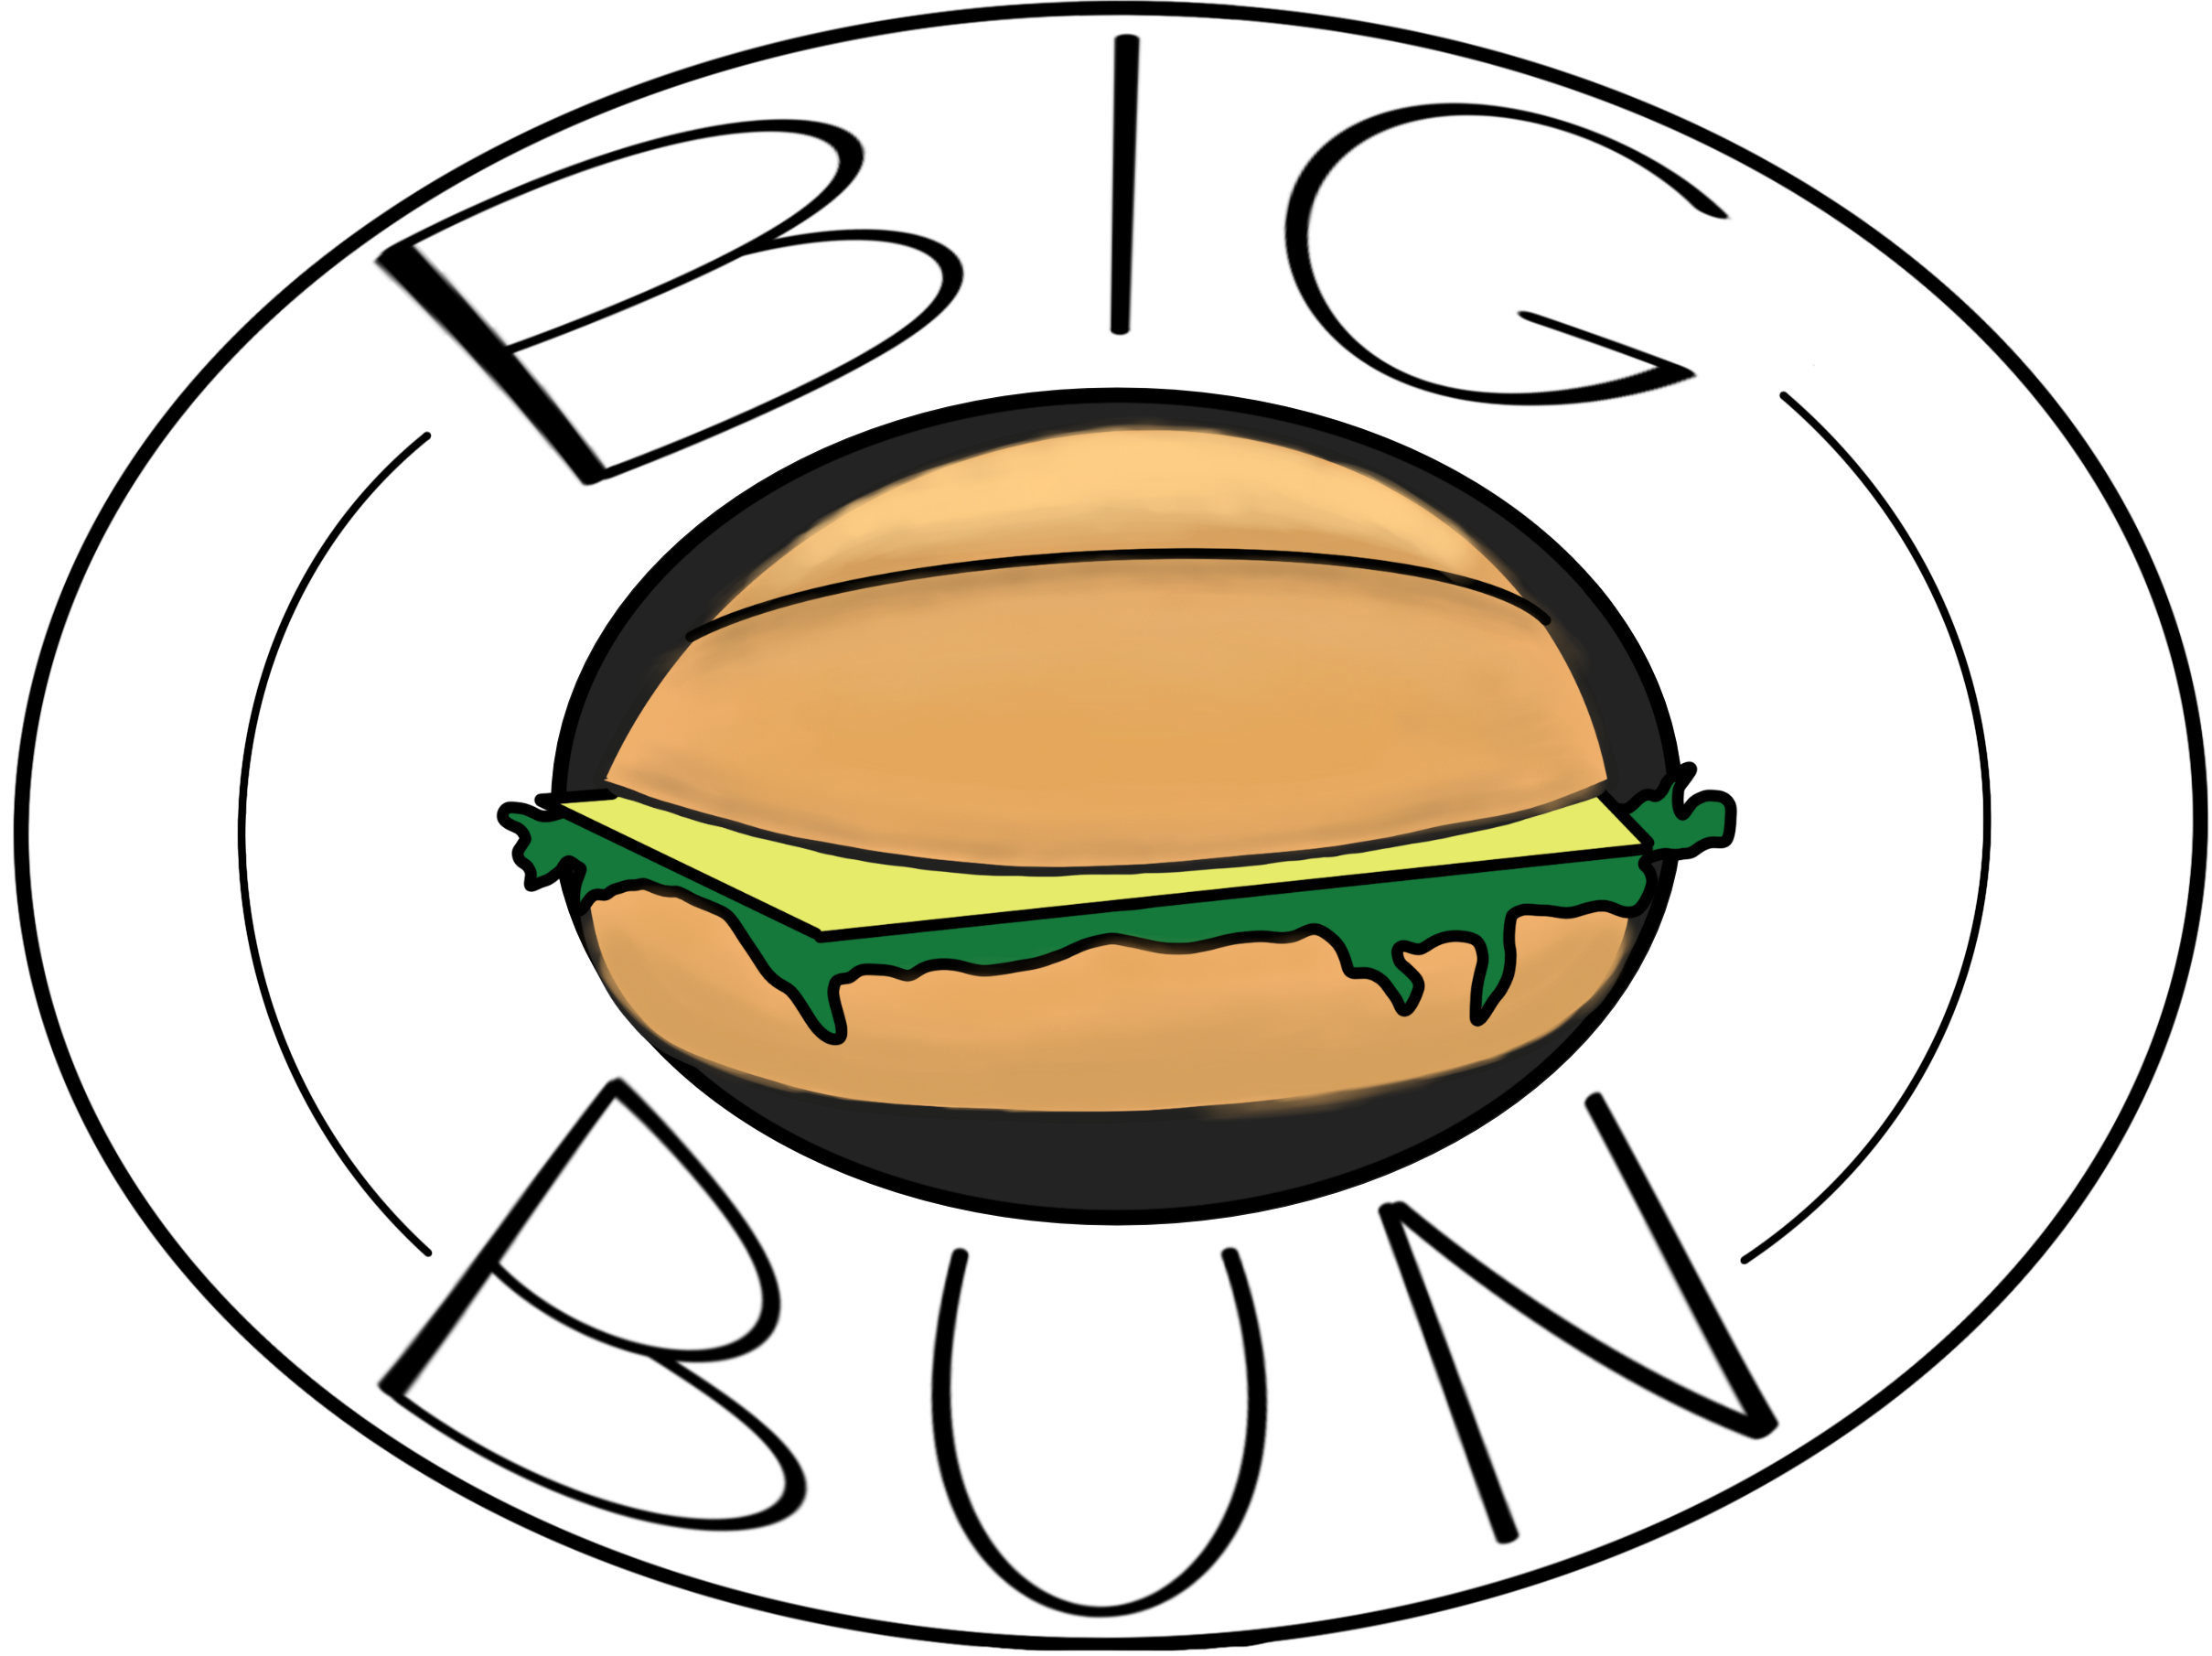
\includegraphics[width=3cm]{images/figures/big_bun_logo.png}
\end{wrapfigure}
It is three in the morning at the regional \textit{BigBun} bakery. Though the
population is still asleep, the work is already taking its course here.
BigBuns supplies a large part of the region with fresh baked goods every
morning. Thousands of residents in the region enjoy the rolls that are
produced in this factory every day. At BigBun however, not only bread and rolls
are being made. Every day, cakes muffins and other sweet pastries leave the
factory to be consumed by the local residents.

The key to the bakery's success is its uncommon means of production. Instead of
one team that prepares one item, e.g.\ a chocolate cake, the production is
split into many small parts. First, multiple small teams prepare the doughs.
Due to the factory's high variety of baked goods, a set of base doughs
consisting of sponge, sourdough, puff pastry and yeast dough are consistently
being produced. Next to the in-house dough production, BigBun also produces its
own fillings and toppings for cakes and prepares the ingredients that go into
the making of their breads and rolls. Depending on the item that is then formed
using one of these doughs, the necessary parts are put together. In order to
e.g.\ make a chocolate muffing, a chocolate filling is added to the sponge base
dough. After baking, an additional chocolate topping is added to make the
muffing even more chocolaty.

Even though so many customers get their baked goods from BigBun's factory, the
packaging floor in the bakery is relatively empty. After the employees finish a
product, it is continuously packaged and labelled with the production date.
Next, the packaged products are shipped to the local baking shops without any
further interventions by the employees working on the production floor. Once
the trucks are loaded, the drivers are instructed to ship the baked goods off
as fast as possible; only then the freshest quality can be guaranteed.

At eight in the morning, Maria gets on her bike. It is Friday and she only has
to be late in at work. After a short ride, she reaches her local baking shop,
gets off her bike and buys two rolls. They taste as good as always even if she
never knew what went into making them; or maybe that's why they taste so great.

\rule{2cm}{0.4pt}

Even though a healthy breakfast surely contributes to the field of computer
science, this thesis examines the workings of microservices that are being
continuously deployed. In the story above, every baking product represents a
microservice architecture. The parts, e.g.\ a topping and filling, that go into
the making of a product, e.g.\ a cake, can be interpreted as individual
microservices. The packaging of products can be directly translated the
packaging of microservices into Docker images. The speed at which the baked
goods are delivered to shops in the area can also be compared to the speedy
continuous delivery of microservices that this thesis strives to explore.
Lastly, the goal is that the production and delivery processes are entirely
transparent for consumer; regardless of whether the consumer uses baked goods
or virtual services.

\todo[inline]{Add explanation of the thesis' structure.}

%! TEX root = ../../main.tex

\subsection{Methodology: Design Science Research}%
\label{sub:Design_Science_Research}

When designing the optimal information system that is able to continuously
deploy microservices, the obvious outcome is a practical model. This model is
embedded in some technical environment but may not contribute any scientific
findings. That is the reason why this thesis uses the \ac{DSR} approach for
designing information systems. \ac{DSR} is an conceptual framework that can be
applied to any research project. It defines seven principal guidelines that
govern the way research should be conducted. This section will explore the
workings of \ac{DSR} and how it will be utilised in this research endeavour.

In general, the goal behind \ac{DSR} is to design \ac{IT} \textit{artefacts}.
An artefact can not only be an instantiation, e.g.\ a software prototype, but
can also be a construct, model and method that is utilised in the development
and usage of information systems \autocite[p.
82]{VonAlanDesignscienceinformation2004}.

The creation of artefacts is regulated by seven guidelines. These guidelines
assure that the requirements for the conducted research are apprehensible for
both the researcher as well as the reader \autocite[p.
82]{VonAlanDesignscienceinformation2004}.

\LTXtable{\textwidth}{tables/design_science.tex}

Table~\ref{tab:design_science_guidelines} lists these guidelines. The intensity
to which the guidelines are enforced can be varied according to the respective
research project. However every guideline should be addressed in some form
\autocite[p.  82]{VonAlanDesignscienceinformation2004}. 

\ac{DSR} also defines a fundamental development cycle. Figure
~\ref{fig:design_science_cycles} shows this cycle embedded inside the \ac{DSR}
\textit{components}. The environment component provides the context, e.g.\ the
research question, for any given research. It consists of all entities acting
inside of the environment. All designed artefacts have to be tested inside the
environment in order to assure that they really solve the identified problem
\autocite[p. 89]{HevnerThreeCycleView2007}.

\begin{figure}[H]
\begin{center}
  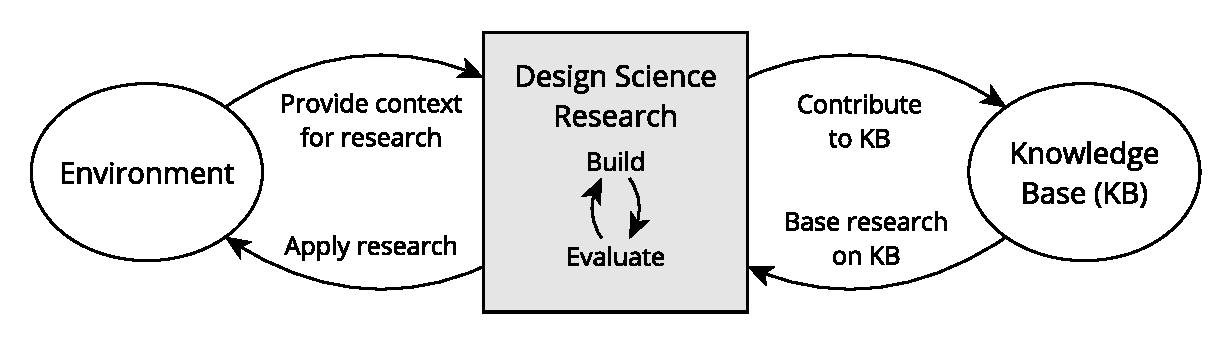
\includegraphics[scale=0.7]{images/figures/design_science_cycles.pdf}
\end{center}
\caption[Simplified interaction model between the environment, knowledge base and Design Science Research.]{Simplified interaction model between the environment, knowledge base and Design Science Research (adapted from \autocite[Fig. 1]{HevnerThreeCycleView2007}).}
\label{fig:design_science_cycles}
\end{figure}

When building artefacts, guideline seven states that any research has to be
conducted rigorously. To achieve this, theoretical foundations as well as
methodologies from the knowledge base can be used \autocite[p.
88]{VonAlanDesignscienceinformation2004}. After an artefact is fully designed,
the findings have to be contributed to the knowledge base; either in the form
of the artefact itself, foundations or methodologies.

The actual development cycle consists of building an artefact and evaluating it
iteratively. Each time this cycle is executed the artefact improves. Such an
evaluation can e.g.\ be performed in an experiment \autocite[p.
91]{HevnerThreeCycleView2007}.

In most cases, an artefact does not represent a complete information system. It
much more tries to capture the ideas, methods and processes that are needed to
design and use an information system \autocite[p.
83]{VonAlanDesignscienceinformation2004}.

In this thesis, for each \href{link:problem_domains}{problem domain} at least
one artefact will be developed. These artefacts answer the research question of
their respective problem domain. 

% TODO: Details zur Verwendung von DSR hinzufügen

